\chapter{مدل طلایی}
\label{chapter:GoldenModel}
\section{مقدمه}
برای ‌انجام یک پروژه، موازی با پیاده‌سازی آن در زبانی مانند وریلاگ،‌ تیم دیگری همان پروژه را در زبانی معمولا سطح بالاتر پیاده‌سازی می‌کنند. این برنامه‌ی پیاده‌سازی شده مدل‌ طلایی نام دارد. از مدل طلایی برای صحت‌ سنجی نتیحه‌ی به دست آمده‌ی مدل اصلی است. خروحی این دو برنامه یکسان است، اما نحوه‌ی پیاده‌سازی این دو لزوما مشابه نیست.
\\ \\
در مدل‌ طلایی ۴ نوع متفاوت از \lr{Skein hash} آورده شده‌است (‌ ۲۲۴ و ۲۵۶ و ۳۸۴ و ۵۱۲  بیت) که همانطور که در مدل  طراحی شده با \lr{verilog} نیز تنها نوع استاندارد  (۵۱۲ بیت)آن پیاده‌سازی شده است , در مدل‌ طلایی نیز تنها توضیحات و مستندات این نوع ارائه خواهد شد.
\\
\begin{center}
	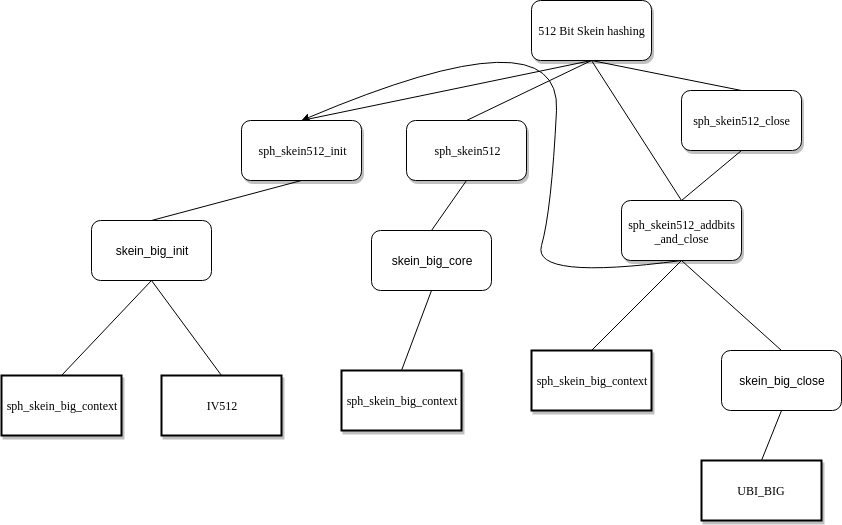
\includegraphics[width=16cm]{images/GoldenModelDocumentation/GoldenModel.png}
\end{center}

\section{پیاده‌سازی الگوریتم}
در شکل بالا تمامی توابع و ساختارهای مورد نیاز  و سلسله مراتب آن‌ها برای نوع ۵۱۲ بیتی الگوریتم آورده شده است , برای توضیح نحوه‌ی اجرای الگوریتم با شروع از
\lr{sph-skein-big-context} سلسله اجرای برنامه توضیح داده خواهد شد.
\\
در این برنامه برای ‌ذخیره و استفاده از هش , از ساختاری به نام \hyperref[subsec:sph-skein-big-context]{\lr{sph-skein-big-context}} استفاده شده است و هدف برنامه اجرای الگوریتم و بدست آوردن درهم‌سازی مورد نظر است.
\\
برای اجرای الگوریتم هش ۵۱۲ بیتی , در سلسله‌ی اجرا از توابع زیر استفاده شده است :
\\
در ابتدا برنامه با ذخیره‌ی مقادیر از پیش تعیین شده  \hyperref[subsec:IV512]{\lr{IV512}} در ساختار معرفی شده شروع به کار می‌کند , و این کار توسط تابع
\hyperref[subsec:sph-skein512-init]{\lr{sph-skein512-init}}
   انجام میگردد.
  \\ سپس با در نظر گرفتن ورودی و سایز این ورودی، اجرای الگوریتم هش  توسط تابع \hyperref[subsec:sph-skein512]{\lr{sph-skein512}}
   شروع می‌شود و این تابع شروع به درهم‌سازی داده‌ی ورودی می‌کند، به این صورت که ابتدا ۵۱۲ بیت ابتدایی را با استفاده از \hyperref[subsec:UBI-BIG]{\lr{UBI-BIG}} هش می‌کند و در ادامه ۵۱۲ بیت بعدی را هش می‌کند تا بیت‌های ‌‌نهایی،‌ که مقادیر آن‌را   در بافر ذخیره می‌کند . مسئولیت درهم‌سازی این بیت ‌های نهایی بر عهده‌ی تابع \hyperref[subsec:sph-skein512-close]{\lr{sph-skein512-close}} است، که این تابع در صورت وجود بیت اضافه در ورودی، با اضافه کردن آن‌ها به دیتای‌ ذخیره‌شده در بافر شروع به درهم‌سازی این بیت‌های نهایی می‌کند ( که این کار را با کمک ماکروی \lr{UBI-BIG} انجام می‌دهد). در انتها نیز مقادیر ساختار هش را به همان مقادیر
 اولیه تغییر می‌دهد.  \\
  حال برای فهم درست از توابع مورد استفاده لازم است نحوه‌ی پیاده‌سازی \hyperref[subsec:UBI-BIG]{\lr{UBI-BIG}} توضیح داده‌شود. تمامی سلسله مراتب طراحی آن در شکل زیر آورده شده‌است.


\begin{center}
  		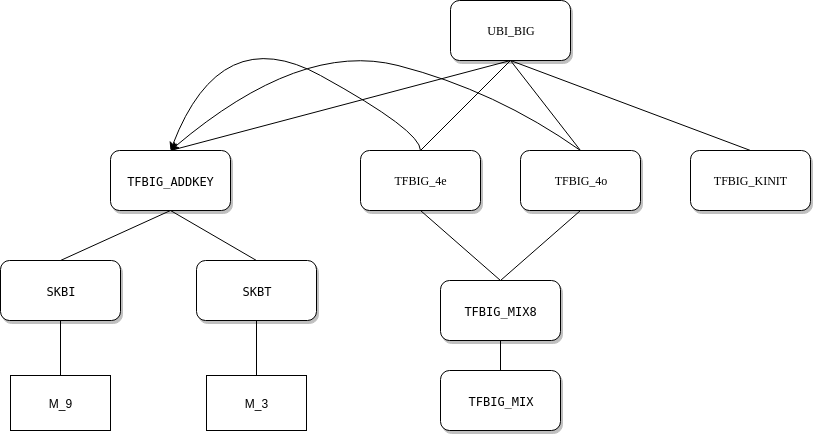
\includegraphics[width=16cm]{images/GoldenModelDocumentation/UBI.png}	
  \end{center}

  

کار این ماکرو درهم‌سازی بلوکی از دیتاست که به عنوان ورودی میگیرد،‌ که این‌کار را با استفاده از نتیجه‌ی درهم‌سازی قبلی و ورودی جدید انجام می‌دهد.

